\documentclass[tikz,border=5mm]{standalone}
\usepackage{pgfplots}
\usepackage{amsmath}
\pgfplotsset{compat=1.18}

% Explicit RGB color definitions
\definecolor{lineblue}{RGB}{0, 0, 128}
\definecolor{linered}{RGB}{214, 24, 66}

\begin{document}
	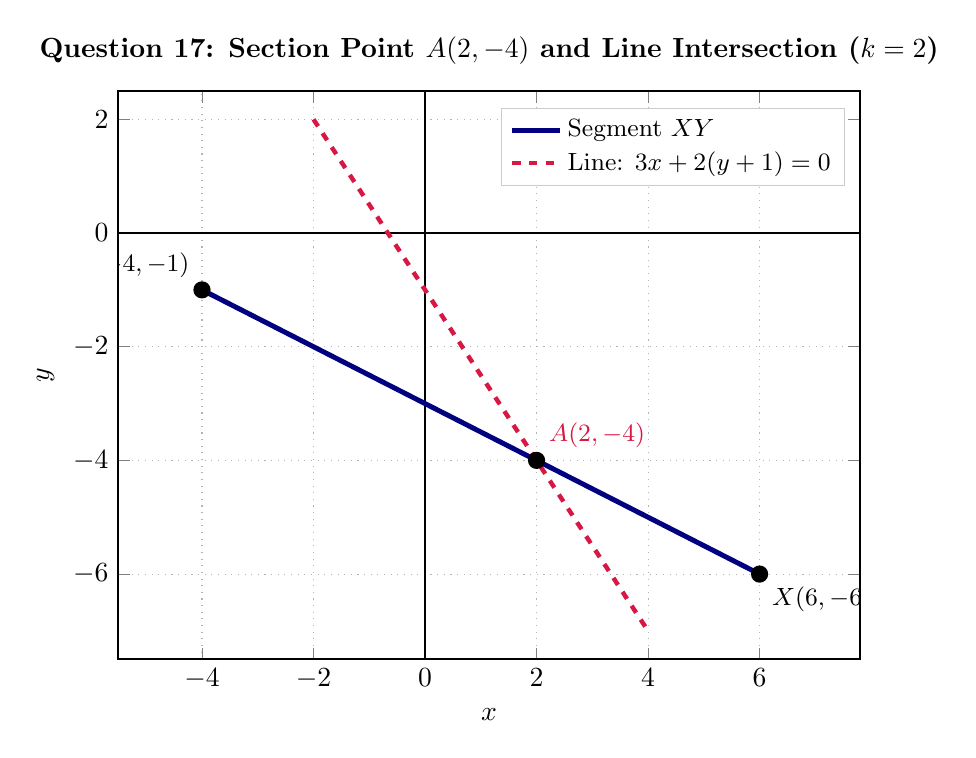
\begin{tikzpicture}
		\begin{axis}[
			width=11cm, height=8.8cm,
			title={\textbf{Question 17: Section Point $A(2, -4)$ and Line Intersection ($k = 2$)}},
			xlabel={$x$}, ylabel={$y$},
			xmin=-5.5, xmax=7.8,
			ymin=-7.5, ymax=2.5,
			xtick={-4,-2,0,2,4,6},
			ytick={-6,-4,-2,0,2},
			grid=both,
			grid style={dotted, gray!60},
			axis line style={black, thick},
			legend cell align={left},
			legend style={at={(0.98,0.97)}, anchor=north east, font=\small, draw=gray!40}
			]
			% Origin axis lines
			\draw[black, thin] (axis cs:0,-7.5) -- (axis cs:0,2.5);
			\draw[black, thin] (axis cs:-5.5,0) -- (axis cs:7.8,0);
			
			% Segment XY
			\addplot[lineblue, line width=1.8pt] coordinates {(-4,-1) (6,-6)};
			\addlegendentry{Segment $XY$}
			
			% Line: 3x + 2(y + 1) = 0  =>  y = -1.5x - 1
			\addplot[linered, dashed, line width=1.6pt, domain=-2:4] {-1.5*x - 1};
			\addlegendentry{Line: $3x + 2(y + 1) = 0$}
			
			% Point Y(-4, -1)
			\node[circle, fill=black, inner sep=2.2pt] at (axis cs:-4,-1) {};
			\node[above left=1pt, font=\small] at (axis cs:-4,-1) {$Y(-4, -1)$};
			
			% Point X(6, -6)
			\node[circle, fill=black, inner sep=2.2pt] at (axis cs:6,-6) {};
			\node[below right=1pt, font=\small] at (axis cs:6,-6) {$X(6, -6)$};
			
			% Section point A(2, -4) with red label
			\node[circle, fill=black, inner sep=2.2pt] at (axis cs:2,-4) {};
			\node[above right=1pt, font=\small, text=linered] at (axis cs:2,-4) {$A(2, -4)$};
		\end{axis}
	\end{tikzpicture}
\end{document}